\documentclass[]{rsos}%%%%where rsos is the template name

%%%% *** Do not adjust lengths that control margins, column widths, etc. ***


%%%%%%%%%%% Defining Enunciations  %%%%%%%%%%%
\newtheorem{theorem}{\bf Theorem}[section]
\newtheorem{condition}{\bf Condition}[section]
\newtheorem{corollary}{\bf Corollary}[section]
%%%%%%%%%%%%%%%%%%%%%%%%%%%%%%%%%%%%%%%%%%%%%%%



\begin{document}

%%%% Article title to be placed here
\title{Survival depends critically on predator detection in zebrafish larvae}

\author{%%%% Author details
Arjun Nair, Christy Nguyen, and Matthew J. McHenry}

%%%%%%%%% Insert author address here
\address{Department of Ecology and Evolutionary Biology\\
University of California, Irvine\\
321 Steinhaus Hall\\
Irvine, CA 92697}

%%%% Subject entries to be placed here %%%%
\subject{Animal behavior, biomechanics}

%%%% Keyword entries to be placed here %%%%
\keywords{Game theory, locomotion, predation, sensing, strategy}

%%%% Insert corresponding author and its email address}
\corres{Matthew J. McHenry\\
\email{mmchenry@uci.edu}}



%%%%%%%%%%%%%%% End of first page %%%%%%%%%%%%%%%%%%%%%

\maketitle

%%%%%%%%%% Insert the texts which can accomdate on firstpage in the tag "fmtext" %%%%%

%\begin{fmtext}


\linespread{1.6}\selectfont %Doublespacing


\section*{Abstract}
Predation is a fundamental interaction between animals, yet it is largely unclear how prey survive encounters with predators.
Using experiments and game modeling, we examined the relative contributions of sensing and locomotion to the survival of larval zebrafish preyed upon by older fish of the same species.
High-speed 3D kinematic measurements of one prey and one predator in an aquarium established the probability distributions of behavioral parameters for both fish.
These measurements provided the basis for events in a game model that predicted the trajectories of predator and prey. 
Upon verifying that the model could replicate the frequency distribution of the number of strikes that prey survived, we conducted a sensitivity analysis to determine which parameters had the greatest influence on prey survival.
This revealed a strong dependency of survival on the response distance and escape speed of prey. 
For example, prey were half as likely to survive if they responded to predators at a distance that was 50\% closer than what was observed.
Escape speed also affected survival, but only through a reduction to less than 50\% of observed values.
The escape direction, predator's speed, and strike distance were all found to have a negligible effect on prey survival. 
Therefore, predator detection is the key metric of performance that distinguishes the survival of larval fish in a piscivorous encounter.
This finding has broad implications for the ecology and evolution of fishes.



\section{Introduction}

The interaction between predator and prey is fundamental to the ecology and evolution of a broad diversity of animals.
For this reason, it is commonly argued that the survival of evasive prey depends on faster or more maneuverable locomotion in biomechanical studies (\hl{CITE}).
The rate and force of predatory strikes are similarly considered important factors (\hl{CITE}) and the ability of prey to sense an approaching predator is often emphasized in studies on behavioral ecology (\hl{CITE}) and neurophysiology (\hl{CITE}).
However, it is rare that these factors are compared in their importance to the outcome of interactions between predators and prey. 
The key traits that distinguish successful predators and prey are consequently unclear. 
The aim of the present study was to determine what factors are most important in determining the survival of fish that are preyed upon by larger fish.

Much of the challenge in the study of predator-prey interactions stems from the coupled nature of the problem . . . \hl{cite Paolo's stuff, ...}

Game theory offers an analytical toolkit for studying the strategic implications of locomotion and sensing . . .
\hl{cite Weihs' paper, Alberto's paper, Casas...}
Differential game theory, as it has been applied to predator-prey interactions, is purely deterministic and consequently offers the opportunity to resolve optimal strategies by analytical mathematics. . .

The present study addressed the strategic importance of sensing and locomotion with a combination of experiments and mathematical modeling. 
High-speed kinematics were recorded of swimming by a single zebrafish larva as it was pursued by an adult predator of the same species, as in previous studies \cite{Stewart:2014cma, Soto:2015cj}.
Descriptive statistics of these interactions were used to characterize the probability of behavioral actions by both the predator and prey.
These findings provided the basis of a game model that was used to simulate the conditions of our experiments. 
Once verified, an analysis of this model was performed to evaluate the sensitivity of prey survival on the behavioral parameters of the predator and prey.

\hl{NOTE:Citations are stored in the ref.bib file.  You can copy and paste citations from Papers as a "BibTex Record"}

\section{Material and methods}

\subsection{Animal husbandry}
All experiments were conducted on zebrafish (\textit{Danio rerio}, Hamilton 1922), where larvae (5 -- 7 days post fertilization, dpf) were preyed upon by older fish of the same species. 
To examine how these interactions vary with the size of the predator, we performed one set of experiments using adult ($\geq 9$ months old, $\SI{3.4}{\cm} \pm \SI{0.5}{\cm}$) predators and another using juveniles  ($3-4$ months old, $\SI{2.0}{\cm}  \pm  \SI{0.4}{\cm}$). 
Although similar in shape, adults were significantly larger in body length and gape diameter than juveniles ($P \ll 0.001$, One-way ANOVA, $N = 19$).
\todo[fancyline]{MJM:What were the values for gape diameter?} 
All fish were bred from wild-type (AB line) colonies housed in a flow-through tank system (Aquatic Habitats, Apopka, FL, USA) that was maintained at $\SI{28.5}{\celsius}$ on a 14:10 h light:dark cycle. 
To culture larvae, the fertilized eggs from randomized mating were cultured according to standard techniques \cite{Westerfield:UXiBrEuA}.
Predators were fasted for a period of 7 -- 14 days prior to an experiment to motivate feeding.


\subsection{Kinematics}
We arranged the lights and cameras for high-speed recordings of both fish with high-contrast images. 
The hemispherical aquarium ($\oslash = \SI{8.5}{\cm}$) was composed of white acrylic, which served as a translucent diffuser of the IR illumination (940 nm) provided by three lamps (CM-IR200-940, CMVision, Houston, TX, USA), positioned below (Fig. \ref{fig_setup}a). 
These lamps provided high-intensity illumination that was invisible to the fish (\hl{CITE}), while visible illumination at low intensity was provided by overhead fluorescent lights.
Each camera (FASTCAM Mini UX50, Precision Photron Inc., San Diego, CA, USA) was fitted with a with a 55mm lens (f/2.8 Micro Nikkor AIS, Nikon Inc., Melville, NY, USA) and positioned at a distance that viewed the entire aquarium. 
The cameras were distributed above the aquarium to allow both fish to be viewed by at least two cameras when the fish were positioned close together.
The cameras were synchronized to record at 1000 fps (at 1280 x 1024 pix) with a common TTL end-trigger and controlled with the manufacturer's software (PhotronFASTCAM Viewer).

Predation experiments were performed by recording the swimming of one predator and one prey fish in a hemispherical aquarium (Fig. 1A). 
Experiments were set up by placing the fish on opposite sides of a partition.
Following a 15 min acclimation period, each experiment began by lifting the partition and ended when the predator successfully ingested the prey.
We recorded $\sim \SI{0.5}{\s}$ before the first predatory strike and ended at $\sim \SI{0.5}{\s}$  after the prey was captured.

The 3D kinematics of both fish were measured from the video recordings. 
The cameras were calibrated by recording a body with 48 landmarks of known relative position that was placed in the center of the aquarium.
Manually selecting the position coordinates from the view of the three cameras provided the basis for a direct-linear transform (DLT), which was calculated using  `Digitizing Tools' software in Matlab (2015a, MathWorks, Natick, MA, USA) \cite{Hedrick:2008wz}.
Using a custom script in Matlab, we found the body positions of predator and prey fish by manually selecting landmarks from two camera views and using the DLT to find the coordinates in 3D space.
For the predator, we found the position of the two eyes from which we calculated a mean position that approximated the buccal cavity (Fig. \ref{fig_setup}a).
The rostrum and posterior margin of the swim bladder were found on the prey's body, which is a position that approximates the center of mass \cite{Stewart:2010ig}.
We acquired the landmark positions at four key events in the interactions between predator and prey: (1) when the predator fish initiated an approach, when the predator (2) began and (3) completed suction feeding and (4) at the initiation of the prey's escape response.


\subsection{Descriptive statistics}

Descriptive statistics were used to characterize the probability of actions by the predator and prey during predation experiments.
The predator-specific parameters consisted of the strike distance ($s$), the proximity from the prey at which a strike was initiated, and the strike duration ($\tau$), which is the period between the opening and closing of the mouth during suction feeding. 
For the prey, we found the reaction distance ($l$), which is the proximity from the predator at which the escape response is initiated.
The escape was additionally characterized by the the escape angle ($\theta$), the angular change in heading from the resting, and the escape duration.
The escape duration ($\eta$) included the period for all stages of the C-start and subsequent undulatory swimming, until the larva ceased motion.
The frequency distribution for each parameter was calculated for the interactions of all experiments and found to be well-approximated by the following log-normal probability density function:
%
\begin{equation}%%% Equation lognormal distribution
f(x) = \frac{1}{x\sigma \sqrt{2 \pi}} \text{exp} \left[ -{\frac{(ln(x)-\mu)^2}{2\sigma ^2}} \right],
\label{eqn_lognorm}
\end{equation}
%
where $x$ is a particular behavioral parameter, $\mu$ is the log mean, and $\sigma$ is the log standard deviation. 
We determined best-fit values for $\mu$ and $\sigma$ for each behavioral parameter by maximum-likelihood (the 'fitdist' function in Matlab).

The probability that the strike of a zebrafish predator is successful depends critically on the distance between the mouth and the prey \cite{Stewart:2013bha}.
The capture probability (i.e. the ratio of captures to strikes) was measured as a function of distance, divided into intervals of ???, for all experiments.
This probability $(C)$ was well-characterized by the following sigmoidal function:
%
\begin{equation}%%%Equation for sigmoid function
C(d) = \frac{1}{1+e^{-r(d-d_0)}},
\label{eqn_sig} 
\end{equation}
%
where $d$ is the distance between predator and prey, $d_0$ is the decay distance, and $r$ is the decay rate. 
The best-fit values for $d_0$ and $r$ were determined by least-squares (the 'sqcurvefit' function in Matlab).

The results of experiments with adult fish predators were compared with the results for juvenile predators.
Because our measurements failed to conform to normal distributions, we performed these comparisons with non-parametric statistics. 
For comparing probability-density functions (Eqn. \ref{eqn_lognorm}) and capture probability (Eqn. \ref{eqn_sig}), we used a two-sample Kolmogorov-Smirnov test (i.e. KS-test) (\hl{CITE}). 


\subsection{Game-theory model}

A pursuit-evasion game model was developed to simulate the conditions of our experiments. 
This game predicts the 2D motion of a predator (i.e. pursuer) and prey (i.e. evader) according to algorithms that are specific to the behavioral state of each of these agents (Fig. \ref{fig_setup}b). 
\todo[fancyline]{MJM:I was wrong about what tense works for the model.  I now see how the present tense can sound less awkward than past tense.} 
The predator's states are Tracking (T) and Striking (S) and the prey's are Resting (R) and Escaping (E). 
The duration of states, probability of transitioning between states, and probability of capture are determined by random-number generators with probability distributions and range of values that match the results of our kinematic measurements.
Therefore, the game treats the predator and prey's actions as probabilistic, but each outcome of the interaction also depends on the determinism of the kinematics of the two agents.
We developed a solver for this game, scripted in Matlab, that calculates the motion of both agents and their behavioral states and consequently finds the payoff, the ultimate score for a game model \cite{Isaacs:1965uz}, as the number of strikes before capture.

A predator begins the game in the Tracking state, where it moves at an approach speed $U$ with a direction that is always headed toward the prey, with perfect information about the prey's position (Fig. \ref{fig_setup}b). 
In this state, the predator is capable of tracking the motion of the prey after a delay $\lambda$.
During periods of prey motion, the direction of predator swimming was calculated with a fixed time step of \SI{5}{\ms}.  
The predator transitions into the Striking state when the prey is within a value for strike distance ($s$), which is determined \textit{a-priori} by the generation of a random value (using the `random' function in Matlab) from the log-normal probability-density function (Eqn. \ref{eqn_lognorm}) for measured values of $s$.
The capture probability for a particular strike depends on the distance between the agents in the middle of a strike, according to our measured parameter values for this relationship (Eqn. \ref{eqn_sig}).
Our simulation uses this relationship to generate a random value from this distance-specific probability to find the range of a strike, with the prey considered captured if it is within that range.
The game ends if the strike is successful, otherwise the predator reverts to the Tracking state after completion of the strike duration ($\tau$).
Single values for the approach speed and predator delay were used for all simulations (Table \ref{table}), determined by trial and error and were found to approximate the mean values observed in prior studies \cite{McHenry:2005tc, Stewart:2013bha}. 

The game model simultaneously determines the actions of the prey fish (Fig. \ref{fig_setup}b).
The behavior of prey was modeled with Resting and Escaping states because we presently found that larval zebrafish generally remain still between periods of rapid swimming initiated by an escape response, as reported previously \cite{Stewart:2013bha, Stewart:2014cma}. 
The prey begins each game in the Resting state, where is it motionless at a distance equal to the aquarium diameter ($\oslash = \SI{8.5}{\cm}$) at a random radial position with respect to the predator's heading.
After a latency ($\chi$) \cite{Nair:2015gk}, the prey transitions into the Escaping state when the predator moves within the reaction distance ($l$).
The prey follows a straight path in the direction of the escape angle ($\theta$) during the Escaping state, and varies in speed according to a saw-toothed function of time, where the escape speed ($u$) is achieved at 20\% of the escape duration $\eta$).
The reaction distance, escape angle, and escape duration are determined by random-numbers with probability density functions matching experimental measurements, similar to the actions of the predator.
The escape angle is defined with respect to the prey's frame of reference, with $\theta =  \SI{0}{\degree}$ corresponding to straight-ahead motion and $\theta = \SI{90}{\degree}$ corresponding to a perpendicular turn.
The escape direction ($\upsilon$) is the probability that this angle is directed away from the predator and was previously measured \cite{Stewart:2014cma}.

This model abstracts many aspects of the complexity of predator-prey interactions in the interest of establishing a predictive first-order approximation.
It assumes that the dynamics may be reasonably approximated with two-dimensional motion and does not bound that motion by the dimensions of an aquarium. 
Simulations were stopped if prey successfully escaped on 20 occasions, which reflected the observed maximum and guarded against an errant simulations from executing for an infinite duration.
The model's probabilistic approach considers the effects of biomechanics and neurophysiology without articulating those elements.
For example, capture success is treated as a distance-specific probability (Eqn. \ref{eqn_sig}) that does not parse the effects of a predator's suction-feeding hydrodynamics, nor the propulsive forces generated by an escaping prey.
The model was tested by comparing the results of simulations against our experimental findings using a Kolmogorov-Smirnov test. 
This test was chosen over a Kruskal-Wallis test because of its emphasis on the shape of the distribution, rather than the median value.  
The number of successful prey escapes before capture for all experiments were compared to the same metric for 1,000 simulations.  

A sensitivity analysis determined which characteristics of the predator and prey behavior have the greatest effect on prey survival. 
This was achieved by running batches of 1,000 simulations with parameters varied individually between -90\% and 100\% of their original values at increments of 10\%.
For parameters described by a probability distribution, the log-mean $\mu$ parameter and the range of values were adjusted by these factors to create a change in the distribution's values.
The effect of these manipulations were assessed by comparing escape probability against the experimentally-validated prediction using a Kruskal-Wallis test. 


\section{Results} %==================================================================

\subsection{Kinematics} %==========
The behavior of both predator and prey were similar whether the predators were juvenile or adult zebrafish.
Prey responded with similar behavior, having indistinguishable differences in escape angle \hl{(KS-test: $P = 00, N = 00$)} and with modest, though significant, differences in reaction distance \hl{(KS-test: $P = 00, N = 00$)} and escape duration \hl{(KS-test: $P = 00, N = ?00$)} (Fig. \ref{fig_PDF}\textit{b--c}). 
For example, prey responded at a mean distance to juveniles \hl{($\overline{l} = \SI{00}{\mm}, N = 00$)} that was \hl{00\%} the value in response to adults \hl{($\overline{l} = \SI{00}{\mm}, N = 00$)}.
The escape swimming of prey continued for a mean duration of \hl{$\SI{00}{\s} (N = 00)$} in response to juveniles and \hl{$\SI{00}{\s} (N = 00)$} in reaction to adults.
Similarly, juvenile and adult predators showed subtle, but statistically significant, differences in strike distance \hl{(KS-test: $P = 00, N = 00$)} and strike duration \hl{(KS-test: $P = 00, N = 00$)} (Fig. \ref{fig_PDF}\textit{d--e}).
On average, strikes by juveniles were initiated at a distance \hl{($\overline{s} = \SI{00}{\mm}, N = 00$)} and 
duration \hl{($\overline{\tau} = \SI{00}{\ms}, N = 00$)} that were \hl{$\sim 00\%$} the values for adult predators \hl{($\overline{s} = \SI{00}{\mm}, \overline{\tau} = \SI{00}{\ms},  N = 00$)}.
Therefore, much of the behavior of predator and prey were similar, despite the fact that the adults were nearly twice the body length of the juveniles.

One major exception in this comparison was in the effectiveness of strikes by suction feeding.
Juveniles did not succeed in capturing prey beyond a distance of \hl{$\SI{00}{\mm}$ ($N = 00$)}, whereas adults were successful at \hl{00-times} that distance \hl{($\SI{00}{\mm}, N = 00$)}.
In the relationship between capture probability and distance (Eqn. \ref{eqn_sig}), the decay distance represents the spatial range at which a predator possesses a high probability of successfully acquiring a prey. 
In this respect, the strike of adult predators exhibited a range that was greater than 3-times the distance of juveniles (Table \ref{table}, Fig. \ref{fig_PDF}\textit{f}).
Therefore, the scale-dependency of suction feeding is the key difference between the predatory performance of juvenile and adult zebrafish.

\hl{Differences between successful escapes and failed escapes in each prey or predator parameter were insignificant (Mann-Whitney U test: P > 0.05, N = see Table 1).
This suggested that neither locomotion or sensing had an significant impact on whether a prey escape attempt was successful or not.}
\todo[fancyline]{MJM:I'm not clear on what data to which the following is referring. Can we dispense with this? I don't think we need to include mention of the failure of conventional stats.}

\hl{This seemed unreasonable since it well known both sensory and motor systems are important for prey survival (CITE). We suspect this discrepancy emerged from the fact that the behavior of predator zebrafish and larval zebrafish were dependent on each other. This led to a coupled system of behavior where there were not strict measurable controls. Therefore, we decided to computationally model the observed predator-prey interactions, allowing the ability to control for various aspects of the predatory encounter.}
\todo[fancyline]{This reads to me like Methods, or maybe Discussion text. Ditch?}


\subsection{Game-theory model} %==========
The trajectories of predator and prey fish followed paths that were qualitatively similar to that predicted by our game model.
In our experiments, predators spent most of their time directed towards prey (Fig. \ref{fig_traj}a). 
The prey were generally motionless, except when escaping from an approaching predator.
This swimming was generally initiated by a fast-start escape response, followed by rapid undulatory swimming.
The predators followed a more circuitous path toward to prey than the motion prescribed by our model (Fig. \ref{fig_traj}b).
However, the temporal sequence of events in the model offers a first-order approximation of the kinematics of live predator-prey interactions.

The model accurately predicted the broad patterns of our experimental results.
This was assessed by the probability that prey survived over a particular number of strikes. 
Prey exhibited the greatest probability of being captured on the first strike and lesser probabilities at greater numbers of strikes (Fig. \ref{fig_traj}c).
Adults were more successful on the first, second and third strikes than juveniles, which exhibited a more-even probability distribution with respect to strike number.
The model was successful in replicating these trends, which were found to be statistically indistinguishable for both adult \hl{(KS-test: $P = 00, N = 73$)} and juvenile \hl{(KS-test: $P = 00, N = 91$)} predators.
\todo[fancyline]{MJM:Does the KS-text give exact p-values, or just a range?  If exact, then report those.}

A sensitivity analysis of the prey parameters revealed that escape speed and reaction distance were the most impactful parameters for prey survival. 
Changes in escape duration, escape direction, and escape angle led to largely insignificant changes in escape probability (Fig. \ref{fig_sense}a). 
However, reaction distance and escape speed had much more substantial effect on escape probability compared to the rest of the prey parameters. 
\todo[fancyline]{MJM:Expand on this point.  By what factors do things change and what degree of change was required in each parameter?}
By increasing the mean value of the reaction distance, escape probability increased significantly. 
\todo[fancyline]{MJM:By how much?}
However, decreasing the mean value of the reaction distance created greater, significant decreases to the escape probability. 
Increasing escape speed did not lead to a significant increase in escape probability and significant decreases to escape probability only occurred when escape speed was reduced by 50\% or more of its original value.

We examined whether escape speed and reaction distance exhibited any interactive effects by conducted a two-dimensional sensitivity analysis.
For this, reaction distance and escape speed were both incrementally changed (Fig. \ref{fig_sense}\textit{b}). 
Escape speed and reaction distance differed in ways that were reflected in our initial analysis (Fig. \ref{fig_sense}\textit{a}). 
At a particular escape speed, increasing reaction distance above the measured value slightly, though significantly, increased the overall escape probability. 
However, a decrease in reaction distance generated large decreases in escape probability (Fig. \ref{fig_sense}\textit{c}). 
\todo[fancyline]{MJM:By how much?}
Decreasing escape speed was the only way to observe significant changes in escape probability when reaction distance was held constant.
  Increasing escape speed while the reaction distance was held constant did not substantially increase escape probability. 
\todo[inline]{MJM:Offer specific examples. e.g. by what factor did probability change for a given combination of changes in speed and distance?}



\section{Discussion} %==================================================================

The present study succeeded in developing a game model for the piscivorous interactions between predator and prey fish. 
This model replicated the broad patterns in the survival of prey (Fig. \ref{fig_traj}\textit{c}) by incorporating measured probabilities of behavioral events (Fig. \ref{fig_PDF}) in formulating predicted kinematics (Fig. \ref{fig_traj}\textit{b}).
A sensitivity analysis of this model revealed that prey survival varies most-substantially on the response distance of prey, which consequently depends on the sensing performance of the prey.
These findings have the potential for broad implications in the biology of fishes and for predator-prey interactions in general.


\hl{This is for later in the Discussion:} The findings of the present study are not anticipate to be generally predictive for all predator-prey interactions. 
Differential game theory illustrates that prey strategy fundamentally depends on the relative magnitude of escape speed relative to the predator \cite{Weihs:1984tb}.
Like many suction-feeding predators \hl{CITE Higham papers}, larger zebrafish approach prey at a relatively slow speed, perhaps in an attempt to control the short-lived and spatially-restricted suction-feeding strike. 
As a consequence, the escape response of larval zebrafish exceeds the speed of the larger predator. 
This permits the prey to escape over a range of directions that are equally successful at maximizing the distance from a predator \cite{Soto:2015cj}.
In this context, it is unsurprising that escape direction has an insignificant effect on prey survival (Fig. \ref{fig_sense}\textit{a}).
However, the same is unlikely to hold true for faster predators.  
Although escape direction matters little in instances when the predators is more than an order-of-magnitude faster than the prey, escape direction conforms to an optimal value in instances with the predator is only slightly faster than the prey \cite{Weihs:1984tb}.
We therefore would anticipate different results for faster predators than the adult zebrafish that we studied.


\section*{Data accessibility}


\section*{Authors' contributions}
The study was designed in collaboration between AN and MJM.
AN and CN performed all experiments and kinematic analysis.
The game model was created by AN, with guidance from MJM. 
The manuscript was written collaboratively by AN and MJM.

\section*{Competing interests}
We declare we have no competing interests.

\section*{Funding}
Insert the Acknowledgment text here.

\section*{Acknowledgments}
Insert the Acknowledgment text here.


%\end{doublespace}

%%%%%%%%%% Insert bibliography here %%%%%%%%%%%%%%
%\section*{References}

\linespread{1}\selectfont %Single spacing

\bibliography{ref}
\bibliographystyle{prsb}   %References the PRSB style file

\pagebreak



\section*{Figures \& Tables}

% AN: How can the mu values for those dimensions given in meters be correct?  Does mu have different dimensions?  Should the units actually be millimeters?

\linespread{1.3}\selectfont %Single spacing

\begin{table}[!h]
\scriptsize
%\small
%\tiny
%\fontsize{6}{6}
\caption{Behavioral parameters and probability distributions}%%%Table caption goes here
\begin{tabular}{lllll}%%%The number of columns has to be defined here
\hline
Variable &State &Adult predator & Juvenile predator\\
\hline
\textit{Predator}& & & & \\
Approach speed, $U$ ($\SI{}{\m\s} ^{-1}$) &T &$U = 0.13$ & $U = 0.05$ \\
Predator delay, $\lambda$ (ms) &T &$\lambda = 10$ &$\lambda = 10$ \\
Strike distance, $s$ (m) &T $\to$ S &$\mu_d$ = -4.980, $\sigma_d$ = 0.448 (\textit{N} = 51) & $\mu_d$ = -5.100, $\sigma_d$ = 0.648 (\textit{N} = 103)\\
Strike duration, $\tau$ (s) &S &$\mu_{\tau}$ = -3.166, $\sigma_{\tau}$ = 0.331 (\textit{N} = 53) & $\mu_{\tau}$ = -3.208, $\sigma_{\tau}$ = 0.399 (\textit{N} = 54) \\
Capture probability, $C$ &S &\textit{r} = \SI{0.573}, \textit{$d_0$} = \SI{5.20}  (\textit{N} = 77) &\textit{r} = \SI{1.99}, \textit{$d_0$} = \SI{1.60}  (\textit{N} = 91) \\ \\
%%
\textit{Prey}& & & & \\
Reaction distance, $l$ (m) &R $\to$ E &$\mu_l$ = -4.546, $\sigma_l$ = 0.587 (\textit{N} = 73) &$\mu_l$ = -4.941, $\sigma_l$ = 0.582 (\textit{N} = 91) \\
Escape angle, $\theta$ (rad) &E  &$\mu_{\theta}$ = 0.144, $\sigma_{\theta}$ = 0.449 (\textit{N} = 206) &$\mu_{\theta}$ = 0.144, $\sigma_{\theta}$ = 0.449 (\textit{N} = 206) \\
Escape duration, $\eta$ (s) &E &$\mu_{\eta}$ = -1.369, $\sigma_{\eta}$ = 0.552 (\textit{N} = 62) &$\mu_{\eta}$ = -1.167, $\sigma_{\eta}$ = 0.5234 (\textit{N} = 91) \\
Escape direction, $\upsilon$ &E &$\upsilon=0.696$ (\textit{N} = 206) &$\upsilon=0.696$ (\textit{N} = 206) \\
Escape latency, $\chi$ (ms) &E &$\chi = 8$ (\textit{N} = 15) & $\chi = 8$ (\textit{N} = 15)\\
Escape speed, $u$ ($\SI{}{\m\s} ^{-1}$) &E  &$u = 0.4$ (\textit{N} = 12) &$u = 0.4$ (\textit{N} = 12) \\\hline
\label{table}
\end{tabular}

T, Tracking; S, Striking; R, Resting; E, Escaping; $\mu$, log mean; $\sigma$, log standard deviation; $r$, decay rate (\SI{}{\per\mm}); $d_0$, decay distance (\SI{}{\mm}).
\end{table}%%%End of the table

\pagebreak

\linespread{1}\selectfont %Single spacing

%The output for figure is:

\begin{figure}[!h]
\centering
	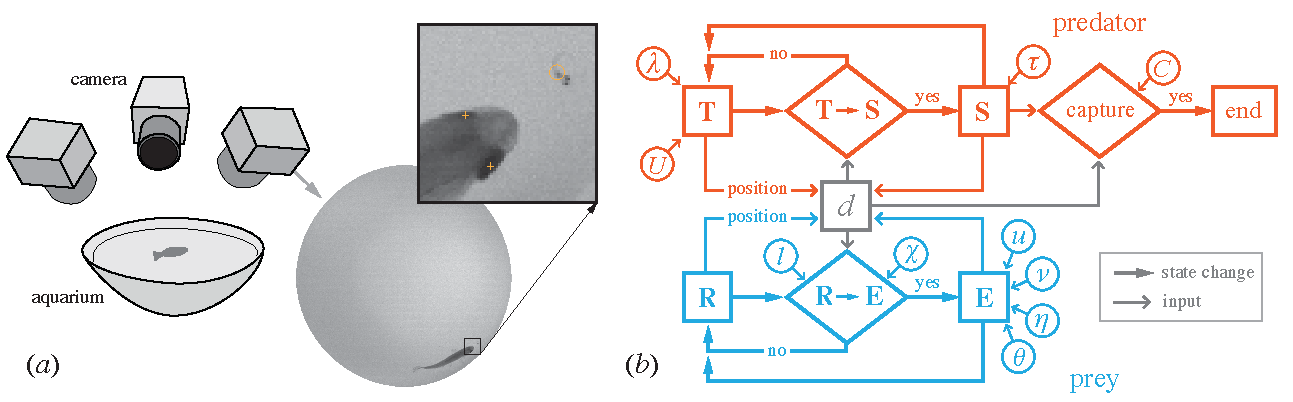
\includegraphics[width=5.5in]{fig_setup}
\caption{Experimental and mathematical techniques for studying predator-prey interactions. 
(\textit{a}) Three high-speed video cameras recorded video of one larval prey and one adult predator fish that were placed in a hemispherical aquarium. 
A representative video frame (cropped to the margin of the aquarium) shows an adult in close proximity to the prey. 
In the inset, white triangles denote the locations of morphological landmarks used to describe the position of the two fish.
 (\textit{b}) A flow chart illustrates the major components of the game model used to simulate the interactions between predators and prey (see Table \ref{table} for symbol definitions and parameter values).}
\label{fig_setup}
\end{figure}

\pagebreak

\begin{figure}[!h]
\centering
	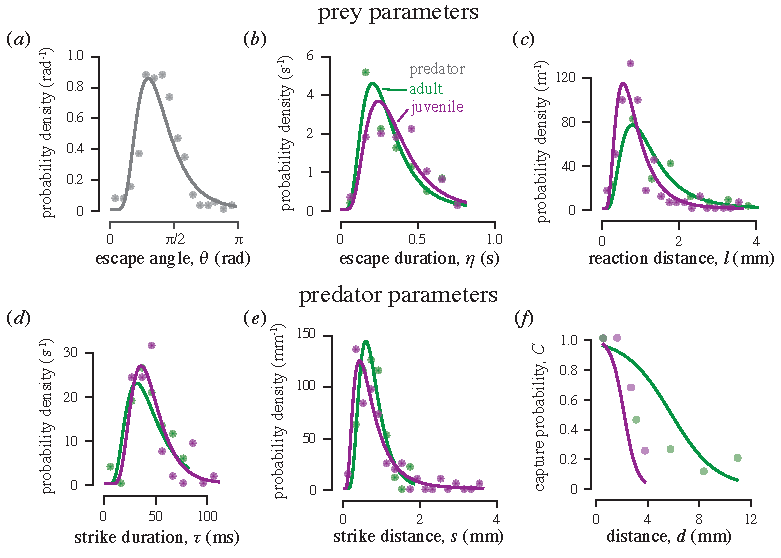
\includegraphics[width=5.5in]{fig_PDFs}
\caption{Descriptive statistics of swimming kinematics. 
(\textit{a-e}) The probability density measurements (circles) and function (Eqn. \ref{eqn_lognorm}) fit for experiments where the predator was a juvenile (purple) or adult (green) predator, which were significantly different, except for escape angle (\textit{a}), shown in gray. 
Parameters were measured from the kinematics of prey (\textit{a-c}) and predators (\textit{d-e}).
(\textit{f}) The capture probability was examined as it varies with distance between the predator and prey (Eqn. \ref{eqn_sig}).  
}
\label{fig_PDF}
\end{figure}

\pagebreak

\pagebreak

\begin{figure}[!h]
\centering
	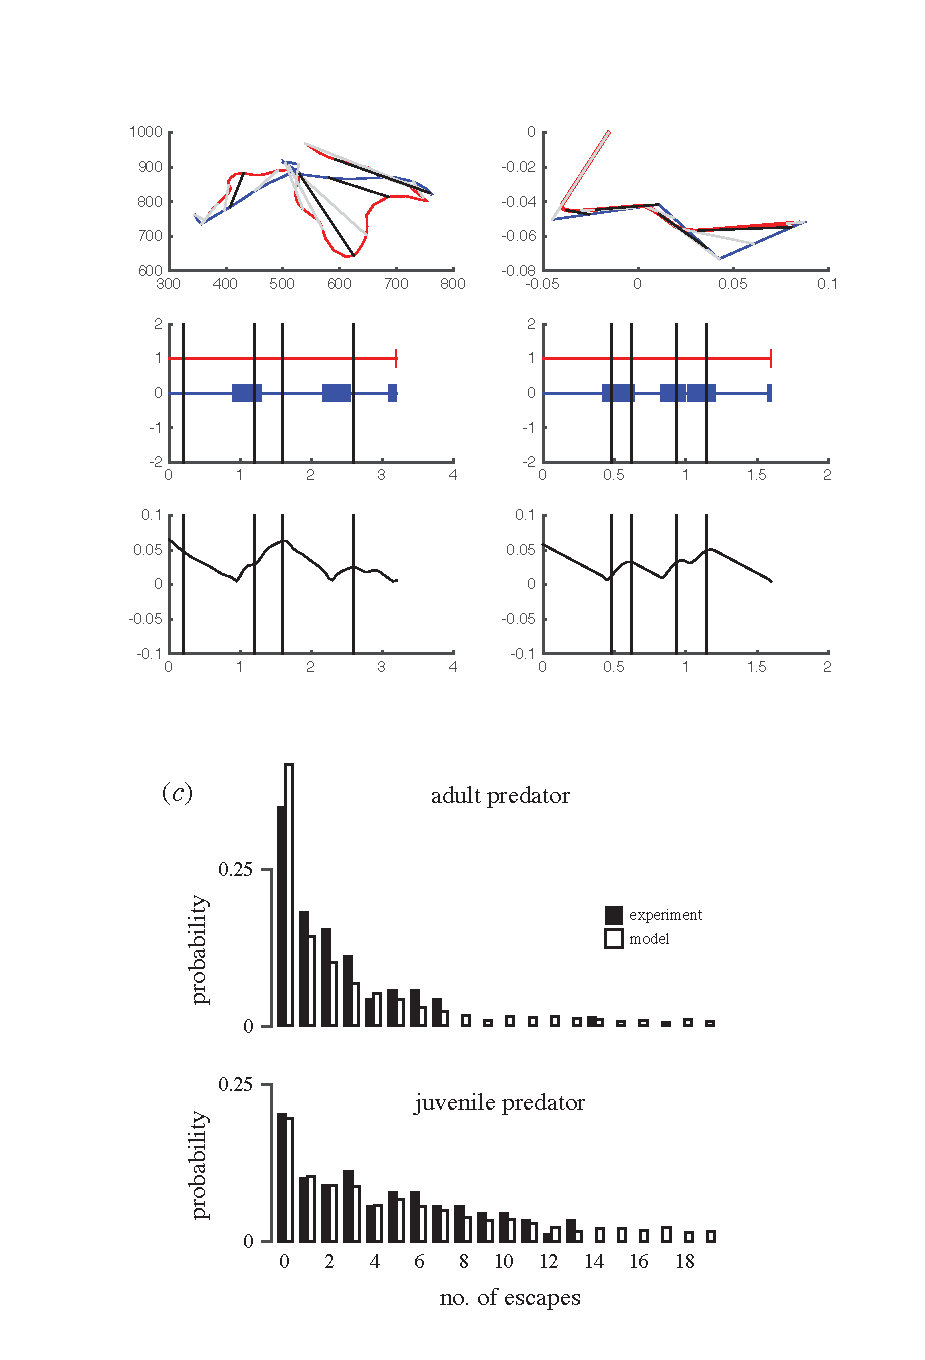
\includegraphics[width=4.5in]{fig_trajectories}
\caption{Comparison between experimental measurements and mathematical modeling. 
(\textit{a}) Trajectories of predator and prey from a representative experiment (left) and simulation (right).
(\textit{b}) Ethograms for these trajectories illustrate the temporal changes in the predator's swimming and strike (left), which are respectively modeled by the T and S (Fig. \ref{fig_setup}\textit{b}) modes (right). 
The prey's behavior while motionless and during escape (left), where modeled with the R and E modes of the model (right).
For both ethograms, the distance between predator and prey are shown and particular moments in the trajectories are highlighted with vertical gray lines.
(\textit{c}) The probability that a prey survives over a particular number of strikes is shown for when the predator was and adult (above) and juvenile (below) for experiments and model simulations.   
}
\label{fig_traj}
\end{figure}

\begin{figure}[!h]
\centering
	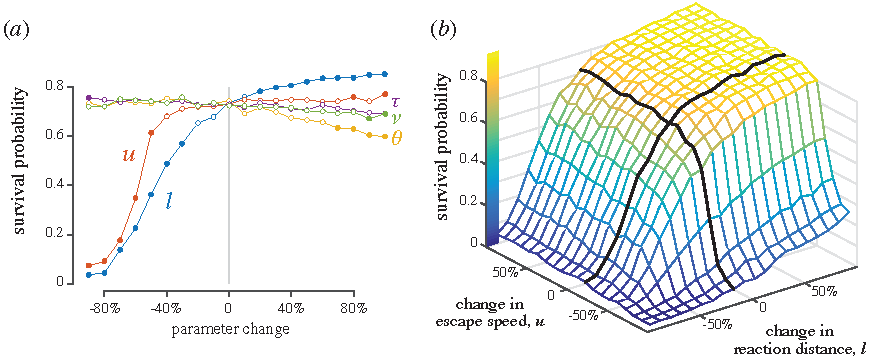
\includegraphics[width=5.5in]{fig_sensitivity}
\caption{Sensitivity analysis of game model to examine the effects of parameter variation on escape probability. 
(\textit{a}) Varying the \hl{log-mean value [MJM:true?]} for the distribution of individual parameters (see Table \ref{table} for parameter definitions and values), with each point representing the result of 1000 simulations. 
(\textit{b}) Variation in escape probability was examined with respect to both escape speed and response distance the same simulation results are shown with respect to changes in escape speed (\textit{c}) and response distance (\textit{d}).
}
\label{fig_sense}
\end{figure}

\pagebreak



\end{document}